\documentclass{article}[11pt]
%Required: You must have these
\usepackage{graphicx}
\usepackage{tabularx}
\usepackage{natbib}
\usepackage{caption}
\usepackage{subcaption}
\usepackage{array}
\usepackage{amsmath}
%\usepackage[backend=bibtex]{biblatex}
\setkeys{Gin}{width=0.8\textwidth}
%\setlength{\captionmargin}{30pt}
\setlength{\abovecaptionskip}{10pt}
\setlength{\belowcaptionskip}{10pt}
\topmargin -1.5cm 
\oddsidemargin -0.04cm 
\evensidemargin -0.04cm 
\textwidth 16.59cm
\textheight 23.94cm 
\parskip 7.2pt 
\renewcommand{\baselinestretch}{1.2} 	
\parindent 0pt

\bibliographystyle{..//..//refs/styles/besjournals.bst}
\usepackage{xr-hyper}
\usepackage{hyperref}
\externaldocument{suppliment}


\usepackage{lineo}
\linenumbers
\title{Biological and environmental drivers of flower-leaf sequence variation in the American Plums (\emph{Prunus}, sect. \emph{Prunocerasus}). }

\author{D.M. Buonaiuto $^{1,2,3,a}$, T.J. Davies $^{4}$, S. Collins $^{4}$, E.M. Wolkovich$^{2,3,4}$}

\usepackage{Sweave}
\begin{document}
\input{plum_manuscript-concordance}
\maketitle
\noindent \emph{Author affiliations:}\\
\noindent $^1$Department of Environmental Conservation, University of Massachusetts, Amherst, Massachusetts, USA. ORCID: 0000-0003-4022-2591\\
\noindent 
$^2$Arnold Arboretum of Harvard University, Boston, Massachusetts, USA.\\
$^3$Department of Organismic and Evolutionary Biology, Harvard University, Cambridge, Massachusetts, USA \\
$^4$Forest \& Conservation Sciences, Faculty of Forestry, University of British Columbia, Vancouver, British Columbia, Canada\\
$^a$Corresponding author: 617.823.0687; dbuonaiuto@umass.edu\\

\section*{Conflict of Interest Statement:}
The authors declare no conflict of interest.

\section*{Author contributions}
DMB, and EMW conceived of the manuscript; DMB and SC collected the data; DMB led the statstical analyses with TJD and EMW; DMB led the writing of the manuscript. All authors contributed to writing and gave approval for the submission.

\section*{Data Availability}
The phenology and trait data collected for this study will be made available and archieved at KNB: The Knowledge Network for Biocomplexity (https://knb.ecoinformatics.org/), at the time of publication.

\pagebreak

\section*{Abstract}
A large number of woody plant species in temperate forests produce their flowers before their leaves emerge each spring. This flower-leaf phenological sequence, known as hysteranthy, proteranthy or precocious flowering is generally described as an adaptation to faciliate wind-pollination, which does not explain why it has also evolved to be common in biotically-pollinated taxa in these regions. 

In this study, we quantified the inter and intra specific varation in flower-leaf sequences in the American plums (\emph{Prunus}, sup.spp \emph{Prunus} sect \emph{Prunocerasus}), an economically and ecologically important clade of insect pollinated woody plants using a large database of digital herbaria specimens. We leveraged these observations to test several hypotheses for the evolution and function of hysteranthy in biotically pollinated taxa by modeling the associations between hysteranthy and several environmental and biological traits related to these hypotheses. We then repeated these analyses for larger genus \emph{Prunus} with trait and phenology descriptions from published guidebooks, to better understand how these phenology-trait associations vary over taxonomic scales.

We found that in both the American plums and larger genus \emph{Prunus}, hysteranthy was associated with aridity and reduced floral display size. These findings support the assertion that hysteranthy may function to temporally partition hydraulic demand between flowers and leaves and reduce water stress, or increase pollinator visibility and reduce selective pressure on increased flower sized.

Our study provides critical insights into the evolution of flower-leaf sequences in biotically pollinated woody plants and paves the way for a continued research agenda regarding function of flower-leaf sequences. Our findings that hysteranthous flowering is linked to both aridity tolerance and pollination success increases the urgency for advancing our understanding phenological sequences as human-caused global change continues to disrupt pollinator services and impact environmental variability. 


\section*{Introduction}
%<<label=numbers, echo=FALSE, results=hide, message=FALSE>>=
%rm(list=ls()) 
%options(stringsAsFactors = FALSE)
%require(brms,quietly = TRUE)
%setwd("~/Documents/git/proterant/investment/Input")
%load("pcerasus.Rda")
%doyeff<-round(fixef(mod.ord.scale.phlyo)[6],digits=2)
%doyints<-round(fixef(mod.ord.scale.phlyo)[6,3:4],digits=3)
\noindent Woody perennials have a unique ability among plants to seasonally begin reproduction prior to vegetative growth. This flowering-first phenological sequence, known as hysteranthy, proteranthy or precocious flowering, is particularly common in temperate deciduous forests around the globe \citep{Rathcke_1985}. A number of studies suggest that this flower-leaf sequence (FLSs) is under selection, and that hysteranthy has functional significance, but the importance of variation in FLSs for maintaining fitness \citep{Gougherty2018,Buonaiuto2020,Guo2014} may vary across functional types and evolutionary clades within the temperate forest biome. With mounting evidence that anthropogenic climate change is driving shifts in flower-leaf sequences \citep{Ma2020:aa}, expanding our understanding of the adaptive benefit of hysteranthy is vital to forecasting the demography and performance of forest communities in an era of global climate change.

\noindent The most common, and well-tested explanation for the evolution of hysteranthy in temperate forests is that it is adaptive for wind-pollination, as leafless canopies increase wind speeds for pollen transport and reduce the likelihood of pollen interception by vegetation \citep{Whitehead1969,Niklas1985}. However, this explanation does not address the widespread prevalence of hysteranthy in biotically-pollinated taxa found in temperate regions. This number is not trivial; a recent analysis found that approximately 20\% of the hysteranthy species in the moist, Eastern Temperate Forests of North America are biotically pollinated \citep{Buonaiuto2020}. 

Several alternative hypotheses to the wind pollination hypothesis have been put forward to explain the advantage of hysteranthy in biotically-pollinated species, but they have not been widely evaluated in the literature. Below, we briefly review these hypotheses and their predictions, and then test these predictions using the American plums (\textit{Prunus} subspp. \textit{prunus} sect. \textit{prunocerasus}), a widespread clade with high variability in flower-leaf sequences as a representitive case-study. Our treatment here both clarifies the hypothesized function of flower-leaf sequence variation in biotically-pollinated taxa, and offers insights into how shifting flower-leaf sequences may impact species demography and distributions as climate continues to change.

\subsection*{Hypotheses of Hysteranthous flowering in biotically pollinated taxa}

\underline{Water limitation hypothesis:} In the dry-deciduous tropics of South and Central America, hysteranthy is common \citep{Rathcke_1985,Franklin2016}, and is regarded as an important adaptation to alleviate water stress by partitioning the hydraulic demand of flowers and leaves across the season in this environment \citep{Gougherty2018,Franklin2016,Borchert1983,Reich1984}. By contrast,
temperate forests are rarely water-limited in the early season during which flowering and leafing occur \citep{Polgar2011}, but there is still considerable variation in water availability in space and time within temperate regions of the globe. Under this hypothesis, the function of hysteranthous flowering in these regions parallels that in the dry tropics---partitioning hydraulic demand across the season to allow hysteranthous species to tolerate increased aridity. If this is the case, we would expect to find hysteranthous taxa in locations that are, on average, drier than their non-hysteranthous relatives.

\underline{Insect-visibility hypothesis:} Hysteranthous flowers are visually conspicuous in the landscape. Thus, as in wind-pollinated taxa, hysteranthy in biotically pollinated taxa may be an adaptation for pollination efficiency as flowering-first species are easier for insects pollinators to locate \citep{Janzen1967}. This hypothesis predicts that hysteranthy should be associated with smaller floral displays, because flower are not obscured by leaves, they are easier to see, and there is weaker selection for increasing floral display size. 

\underline{Fruit maturaturion hypothesis:} There are several aspects of reproductive development that suggest hysteranthy is a by-product for early flowering, driven by development constraints. Hysteranthy may be common in large fruited species that require lots of time to mature their fruits, or in small, early fruiting species that have evolved dispersal syndromes (wind dispersal, non-dormant seeds) that require dispersal early in the season \citep{Primack1987}. In either case, we should expect fruit size to associate with hysteranthy.

Alternative to these functional hypotheses is the assertion that hysteranthous flowering is simply a by-product of selection for early flowering. Species that flower before their leaves inherently flower early in the season. Spring flower phenology is less constrained by prior phenological events than leaf phenology \citep{Savage2019}, which could allow selection to drive flowering into the early season, producing the hysteranthous phenological sequence. Here, there is no specific adaptive advantage to hysteranthy;  selection is not operating on the relative timing of flower and leaf emergence, but rather the absolute flowering time alone. If none of the predictions of the previously stated hypotheses are supported, this is the most likely null hypothesis.

\noindent A significant challenge for robust testing of hysteranthy hypotheses is that most characterizations of flower-leaf phenological sequences are based on expert-opinion verbal descriptions (e.g. ``flowers before leaves" or ``flower before/with leaves"), which make comparisons across taxa, time and space difficult and sensitive to observer bias  \citep[see;][]{Buonaiuto2020}. This problem can be overcome by adopting standardized quantitative measures of plant phenology for observational studies and applying them to historic data records. Herbarium records are an excellent source of data that can be leveraged for quantitative phenological measurements \citep{Willis2017}, but have not be used widely to investigate variability of flower-leaf sequences variation among and within species.

The American plums offer potential for a high resolution investigation of drivers of hysteranthous flowering in taxa that are not easily explained by the dominant wind-pollination hypothesis. The 16 species that make up the section are distributed across the temperate zone of North America and, like the genus \textit{Prunus} at large, are all insect-pollinated, yet show pronounced inter-specific variation in flower-leaf sequences. Species in this section are well represented in herbaria records (Fig. \ref{fig:phylo2}a), making them a tractable group to measure and assess variation in flower-leaf sequences.

\noindent In this study we ask:\\

Do the observed associations between flower-leaf sequence variation and morphological and environmental traits match predicted associations of the hysteranthy hypotheses? 

\noindent First, we used herbaria records to to quantify both within- and across- species level variation in flower-leaf sequences of the American plums, (subspecies  \textit{Prunus}, sect. \textit{prunocerasus}).
Then we combined environmental attributes, biological traits and phylogenetic data in statistical models to interrogate the functional hypotheses for hysteranthous flowering described above. Finally, we compared our findings in this clade to patterns observed in larger genus \emph{Prunus} to better understand how phenology-trait associations vary over taxonomic scales.


\section*{Methods}
\subsection{Quantifying flower-leaf sequence variation}  

We obtained digital herbarium specimens for all members of the section \textit{Prunocerasus} from the Consortium of Midwest Herbaria (CMH) Database \citep{add citation}. To quantify flower-leaf sequence variation within and across species we randomly sampled 200 specimens for each species and scored the phenological development of flowers and leaves using a modified BBCH scale for woody plants \citep{Finn2007}. In total, we evaluated the phenology of 2521 specimens, but only specimens with visible flowers were included in this analysis (n=1009). We reconstructed the phylogenetic relationships among species in this group based on the tree topology in \citet{Shaw:2004aa}. We inferred branch lengths following the method of \citet{Granfen1989}in which node heights are estimated in proportion to number of subtending taxa using the R package ``ape" \citep{Paradis2019}.

To quantify FLS variation, we fit an ordinal, hierarchical, Bayesian, phylogenetic mixed model \citep{Garamszegi2014} to assess the likelihood an individual would be at any given vegetative BBCH phase while flowering. Our model predicted leaf stage (Y, ordinal with up to j categories) as a function of species and additional phylogenetic effects. Because hysteranthy co-varies with flowering time (i.e., flowering first species will generally flower earlier than other species, on average) we included day of observation as an additional predictor. The model is written below:\\

$logit(P(Y \leq j)) &= \alpha_{[j]phylo[i]}+ \alpha_{[j]sp[i]}+ \beta_{day of year[sp[i]]}*X_1+ \epsilon_{i}$\\
  
   \epsilon_i & \sim N(0,\sigma^2_y) \\ 
   
where Y is the ordinal outcome (leaf stage) and j is the number of categories (1,2,...6). $P(Y \leq j))$ is the probability of $Y$ less than or equal to a category $j&=1...j&-1$. $\alpha_{[j]}$ describes an intercept for each category [1,2,...6], while slope $beta_{\text{day of year}[sp[i]]}$ is constant across categories. 
  
  \noindent The influence of the phylogeny $\alpha_{phylo}$ was modeled as follows:\\
  \alpha_{sp} & \sim N(\mu_{\alpha}, COR[\sigma^2_{phylo}]) \\
  
  \noindent The $\alpha$ for species effects independent of the phylogeny was modeled as follows:\\
  \alpha_{sp} & \sim N(\mu_{\alpha}, \sigma^2_{species}) \\

We used our model to predict the likelihood each species would be observed at a given vegetative BBCH stage during flowering at the 0\%, 25\% 50\% and 75\% quantiles of their flowering period. We then developed a flower-leaf sequence index, by assigning a numerical score to each species per seasonal quantile, and summing over the full flowering season. In each seasonal quantile, species received a ``1" if more than 50\% of their probability distribution occurred at the two earliest stages of vegetative phenology---BBCH 0 (``bud development") and BBCH 09 (``bud break")---and a ``0" if not. We summed these values across the season, generating an index from 0 (never hysteranthous) to 4 (hysteranthous through late season (Q75)), where 1&= hysteranthous at start of season, 2&= hysteranthous through early season  (Q25) and 3 &= hysteranthous through mid season (Q50). We also used two alternative indexing schemes ($>$25\% of the probability distribution occurred at BBCH 0 and $>$40\% of the probability distribution occurred at BBCH 0 and BBCH 09) to make sure our result were robust across multiple cutoffs.

\subsection{Evaluating hysteranthy hypotheses}

To test the predictions of the hypotheses we obtained data on petal length and fruit diameter directly from herbarium specimens. To assess aridity tolerance, we computed the average Palmer Modified Drought Index score from 1900-2017 for every \textit{Prunocerasus} specimen in the database (n=2305) from the North America Drought Atlas \citep{Cook2004}. For any specimens that lacked accurate geo-location information, we extracted PDSI values at the county centroid of the herbaria specimen. 

\noindent For our morphological measurements, we sampled an additional 321 specimens and measured the petal length of up to 10 randomly selected petals per specimen (n=2757) using ImageJ image processing software. We also used ImageJ to measure the diameter of fruits on an additional 316 specimens, measuring up to 5 fruit per specimen (n=224).

We then used Bayesian phylogenetic mixed models to test the relationship between flower-leaf sequence index scores and each of the variables. In these models, we modeled species and phylogeny as above. 

The model structure is written below: 

  y_i &= \alpha_{ind/sp[i]} +\alpha_{phylo[i]} + \beta_{hyst.index}*X_{hyst.index} + \epsilon_i\\
  
  \epsilon_i & \sim N(0,\sigma^2_y) \\ %Check this
  
  where Y is observed trait values (PDSI, petal length or fruit diameter), and the slope $\beta_{\text{hyst.index}$ describes the relationship between extended hysteranthy (higher hysteranthy index value) and the trait of interest. \alpha_{ind/sp[i]}  and \alpha_{phylo[i]} describe the species and phylogenetic effects respectively.  We also ran each model using our two alternative FLS indexing approaches to make sure our particular indexing approach was not influencing our results. Though these alternative classification schemes did change the hysteranthy index score for some species (Fig. \ref{fig:plums}), they did not substantially impact the inference from our models (see Tab. \ref{tab:modput} for comparisons).
  
\subsection*{Hysteranthy in the larger genus \textit{Prunus}}

To better understand how the patterns we identified in our in-depth study of the \textit{Pruncerasus} clade scaled across coarser taxonomic resolution we also evaluated the relationship between hysteranthous flowering and hypothesis-related traits in all of the \text{Prunus} species that are native to, or established in North America. For this analysis, we obtained categorical descriptions of flower-leaf sequences and mean estimates of fruit diameter and number of flowers/inflorescence as a proxy for floral investment from the Flora of North America \citep{add citation} for 32 species in the genus.  We extracted PDSI values for all herbaria observation of those species in the Consortium of Midwest Herbaria database (n=23,272) as described above.

 
To account for the influence of evolutionary relationships among species, we reconstructed the phylogenetic relationships in the genus based on the tree topology in \citet{Chin:2014wu}. As as above, we computed branch lengths with the R package ``ape" \citep{Paradis2019}. 

We standardized the units of all predictors to make their effect size estimates for the following model structure directly comparable to each other: 

$logit(P(Y \leq j)) &= \beta_{[j]phylo[i]}+ \beta_{pdsi[sp[i]]}*X_1+\beta_{fruit diamter}*X_2+
+\beta_{floral investment}*X_3+\epsilon_{i}$\\
  
   \epsilon_i & \sim N(0,\sigma^2_y) \\ 
   
   where Y is the ordinal outcome of flower-leaf sequence category (``flowers before leaves",``flowers before/with leaves", ``flowers with leaves" and ``flowers after leaves") and j is the number of categories (1,2,...4). $P(Y \leq j))$ is the probability of $Y$ less than of equal to a category $j&=1,...j&-1$. We modeled the influence of the phylogeny ($\alpha_{phylo}$) as above.

\subsection{Model runs} 
 
We fit all models in the R package ``brms" \citep{Burkner2018} using weakly informative priors, and ran the model on four chains.
For the ``Quantifying flower-leaf sequence variation" and ``Evaluating hysteranthy hypotheses" we ran the models with a warm-up of 3000, and 3500 iterations, and 4000, and 4500 sampling iterations respectively, for a total of 4000 sampling iterations across all chains. For the ``Hysteranthy in the larger genus \textit{Prunus}" model, we used a warm up of 6,000 iterations and 8,000 sampling iterations for a total of 8,000 sampling iterations to maximize the effective sampling size. Model fits was assessed with Rhats <1.01, high effective sample sizes and no divergent transitions.

\section*{Results}
\subsection*{Quantifying flower leaf sequences in the American plums}
We found substantial inter-specific differences in flower-leaf sequences within the American plums (Fig. \ref{fig:ordinals}, \ref{fig:plums}). Flower-leaf sequence patterns were strongly dependent on the day of observation, with observations later in the the flowering season of each species decreasing the likelihood of finding flowers open during early vegetative BBCH phases ($\beta_{doy}$ 0.03, $CI_{50}$ [0.02,0.03] ). Based on our flower leaf sequence index, two species (\textit{P. umbellata}, \textit{P. mexicana}) were likely to be hysteranthous regardless of the time of observation and three species (\textit{P. rivularis}, \textit{P. subcordata}, and \textit{P. texana}) were always most likely to flower after with leaves present (Fig. \ref{fig:phylo2}b). All other species displayed intermediate phenotypes, with five species mostly likely to hysteranthous at the start of the season (\textit{P. alleghaniensis}, \texrit{P. americana}, \textit{P. hortulana}, \textit{P. munsoniana} and \texit{P. nigra}), one species through early season (\textit{P gracilis}) and two species through mid season (\textit{P. angustifolia}, \textit{P. maritima}) (Fig \ref{fig:phylo2}b).

\subsection*{Associations between hysteranthy and environmental and morphological traits}
In the American plums clade, aridity (lower average PDSI) was associated with higher flower-leaf sequence index scores ($\beta$: -0.03 ,$CI_{50}$[-0.05,  0.02] ,Fig. \ref{fig:prunes}a.), suggesting that species that displayed hysteranthous flowering later into their flowering season are found in dryer locations. 

Shorter petal and smaller fruit diameters were also associated with higher flower-leaf sequence index scores ($\beta$: -.21, $CI_{50}$[-0.38 -0.04],$\beta$:-1.40, $CI_{50}$[-1.97 -0.82] respectively, Fig. \ref{fig:prunes}b.,c.). This suggests that smaller fruits and flowers are associated with increased hysteranthy.

At the genus level, there was a positive association between increasing PDSI and inflorescence size and increasing overlap between flowers and leaves (i.e., decreasing hysteranthy, $\beta$: 2.50, $CI_{50}$[1.17, 3.371] and $\beta$ 6.41,$CI_{50}$[3.86, 8.05] respectively, Fig. \ref{fig:genus}a), suggesting that hysteranthy is associated with drier locations and smaller floral displays (Fig. \ref{fig:genus}b). Hysteranthy was associated with larger fruits  ($\beta$: -1.24, $CI_{50}$[-1.95,-0.21], \ref{fig:genus}b)]  though there was high uncertainty around these estimates in our model. 

\section*{Discussion}
Our study provided foundational insights into the evolution of flower-leaf sequences in biotically pollinated plants. Our findings that hysteranthous flowering has potential to be linked to both aridity tolerance and  pollination success through the predictions of the water limitation and insect visibility hypotheses increases the urgency for advancing our understanding phenological sequences as human-caused global change continues to disrupt pollinator services and impact environmental variability. 

\subsection*{Hysteranthy hypotheses}
Using North American \textit{Prunus} species as a case study, our analyses support that flower-leaf sequences are under selection by biological and environmental drivers, and that variation in these patterns across species may reflect adaptive tradeoffs. We found that hysteranthous flowering is associated with smaller floral displays and increased aridity in both the American plum clade of the genus \emph{Prunus}, and more broadly the members of the full genus that are the native or established in North America. While we did not find support for the fruit maturation hypotheses, the relationships between hysteranthy and aridity, and hysteranthy and floral display size support the predictions of the water limitation hypothesis and the insect visibility hypothesis, respectively. 

The support for both the water limitation hypothesis and insect visibility hypothesis highlights that these hypotheses are not mutually exclusive, and could be related. Selection on floral size represents a classic evolutionary tradeoff where larger floral displays may generally be more effective for attracting pollinators but demand more resources, including water, to maintain turgor and reproductive function than smaller ones\citep{Galen:1999vr,Lambrecht:2007ur}. With this trade-off, reproductive displays are often small in harsher environments \citep{}, and hysteranthy could represent a compensatory mechanism that both reduces hydraulic demand while increasing pollination efficiency in these environments.

Studies that have compared the transpiration rates among flowers and leaves provide insights to the potential importance of this seasonal partitioning for maintaining water status. Measurements of water movement (transpiration rates, sap flow, hydraulic conductivity) to flowers range from 20\%-60\% of that of leaves under comparable conditions \citep{Whiley:1988uf,Roddy:2012wn,Liu:2017wg,McMann:2022ww}. This level of additional hydraulic demand can drive loss of stomatal conductance and decrease photosynthetic rates \citep{Galen:1999vr}.
 
Yet, despite this evidence that hysteranthy can reduced hydraulic demand in dry environments it is noteworthy that even the hysteranthous species in the American plum clade are not found in extremely arid locations (mean pdsi values only rangeed from -.48 to 0.2 for species classified as hysteranthous through mid-season or through late season). This is in stark contrast with hysteranthous species in the dry tropics where this phenological syndrome allows  them to tolerate more extreme aridity \citep{Franklin2016}. But the flower-leaf sequences of the hysteranthous species in our study were markedly different from patterns of hysteranthy in these dry-tropics where the water limitation hypothesis developed. While flowering can precede leafout by as much several weeks for species in our focal clade, the process of fruit development, which is also water intensive, occurs when leaves are present. By contrast, in the dry tropics hysteranthous flowering is initiated at the time of leaf drop \citep{Borchert1983,Franklin2016}. This makes it that the full reproductive cycle occurs in the leafless period. The comparatively small window of leafless reproductive development in our temperate clade, may in part, explain why the association we observed between hysteranthy and aridity in our study was relatively weak with high residual variance. Our result suggest that hysteranthy may allow temperate species to occupy marginally drier environments than non-hysteranthous species, but may not facilitate species' persistence under extreme aridity. 

\subsection*{Inter-and intra-specific variation in flower-leaf sequences}
In our study, we developed a novel approach to assessing flower-leaf sequences that scales from quantitative, individual-level observations to species levels characterizations based on empirical likelihood estimates. With this approach, we were able to for the first time quantitatively assess intermediate cases of hysteranthy (ones that are typically described as ``flowers before/with leaves"). Previous studies of hysteranthous flowering have either excluded these cases from their analyses  \citep[e.g.;][]{Gougherty2018} or binned them with the well defined cases \citep[e.g.;][]{Buonaiuto2020}. We found that eight of the thirteen American plum species expressed this intermediate flower-leaf sequence, but by estimating the likelihood of hysteranthy across the growing season with Bayesian methods, our approach identified substantial differences in FLSs among them (Fig. \ref{fig:ordinals}, Fig. \ref{fig:plums}), which allowed us to robustly assess the trait associations related to the hysteranthy hypotheses addressed above.

Our quantitative analysis of the American plums clade revealed that flower-leaf sequences---often described as a species-level trait---are highly variable within species (Fig. \ref{fig:ordinals}, Fig. \ref{fig:plums}). For all members of the clade, the day of phenological observation was a strong predictor of the likelihood that flowers would be visible before the emergence of leaves. In many cases, there was high likelihood that individuals of a species may be observed at different vegetative stages during flowering (Fig. \ref{fig:prunes}, \ref{fig:plums}). This could either suggest high levels of local adaptation in flower-leaf sequences or, alternatively, high levels of plasticity through which flower-leaf sequences respond to interannual variation in environmental conditions. For example---in a given population--- flower-leaf sequences may vary in relationship to interannual variation in precipitation with increasing the time period between flowering and leafout in dry year and decreasing time between these phases in wetter years. Our data did not have the temporal resolution to address this question, but the high levels of within species variation we observed raise important questions about environmental drivers of flower-leaf sequences opperating on both the macro-evolutionary scale we investigated here on individual physiological responses to environmental change. 

Additionally, by related these individual, quantitative observations as ordinal response categories with our hysteranthy index, we were able to consider our results in context with existing categorical, species-level characterizations based on expert opinion. The coherence of inference between our individual based observational approach for the American plum clade and the top-down, categorical data we analyses larger genus \emph{Prunus} is an encouraging demonstration that the categorical, expert opinion-based data can still offer useful insights the the drivers of hysteranthous flowering when higher-resolution data is not available. Our modeled flower-leaf sequences patterns of the American plums also qualitatively agreed with previous characterizations of the the species-level variation in this group \citep{Shaw:2004aa}, indicating that the biological patterns we observed are relatively robust to these methodological choices.

\subsection*{Future directions}

In this study, we focused on a well-studied, and economically important clade of morphologically similar species, that allowed us to control for unmeasured biological variation on our traits of interest. This case-study critically provides a road map to evaluate the role of hysteranthy more broadly in temperate biotically pollinated plant taxa (groups with high interspecific flower-leaf sequence include \emph{Magnolia}, \emph{Rhododendron}, \emph{Acer} and \emph{Cornus}). 

Combining the observational approach we employed in this study, with novel experiments could advance our collective understanding of the adaptive significance of flower-leaf sequences. To test the water-limitation hypothesis, researchers could plant sister-taxa with contrasting flower-leaf sequences in common environments across a gradient of aridity, and evaluate their performance. To test the insect visibility hypothesis, researchers should also consider hysteranthy---and phenology in general---in the more general framework of tradeoffs in pollination biology. The trade off between phenology and pollination investment should not only consider flower size, but also the number of flowers, nectar and pollen reward investment, volatiles between related hysteranthous and non-hysteranthous taxa. The expectation here is that hysteranthous species would invest less resources into these other pollinator attration traits than non-hysteranthous relatives. For a simple experiment to test the pollinator visibility hypothesis, researchers could place hysteranthous and non-hysteranthous individuals in a controlled environment, and systemically release pollinators to observed their preference, search times and foraging behavior. If pollinators are more readily drawn to the hysteranthous individuals, it would suggest that hysteranthy is an adaptive trait for pollinator attraction.

With a better mechanistic understanding of the relationship between flower-leaf sequences and ecological performance in hand, researchers could then use experiments to assess how differences in floral and leaf physiological responses to temperature variation may alter the adaptive benefits of flower-leaf sequences with climate change. The measurement and modeling approaches we developed in our observational study can be readily implemented to analyze data from these experimental settings, representing an important opportunity to unite observations of broad ecological patterns with targeted mechanistic explanations in order to better understand both the evolutionary past and ecological future of flower-leaf sequences in temperate woody plants.




\bibliography{..//..//..//sub_projs/refs/hyst_outline.bib} 

\newpage
\section*{Figures}


\begin{figure}[h!]
  \centering
 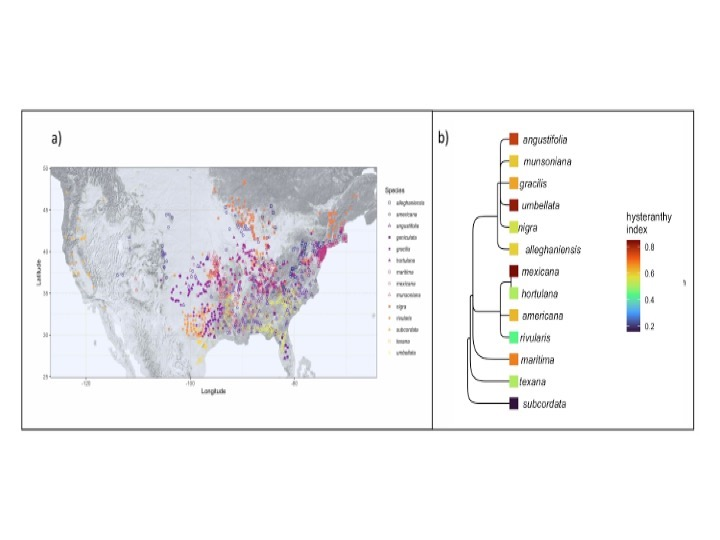
\includegraphics[width=\textwidth]{..//..//Plots/fig1_new.jpg}
    \caption{Geographic distribution and taxonomic relationships among the focal clade Prunocerasus. a) Maps the localities of all the herbaria records used in this study. b) Depicts phylogenetic relationships among the American plums and the duration of their flowering period they are hysteranthous. These categorizations are based on ordinal phylogenetics mixed models. Tree topology is from \citet{Shaw:2004aa}}
    \label{fig:phylo2}
\end{figure}



\begin{figure}[h!]
    \centering
 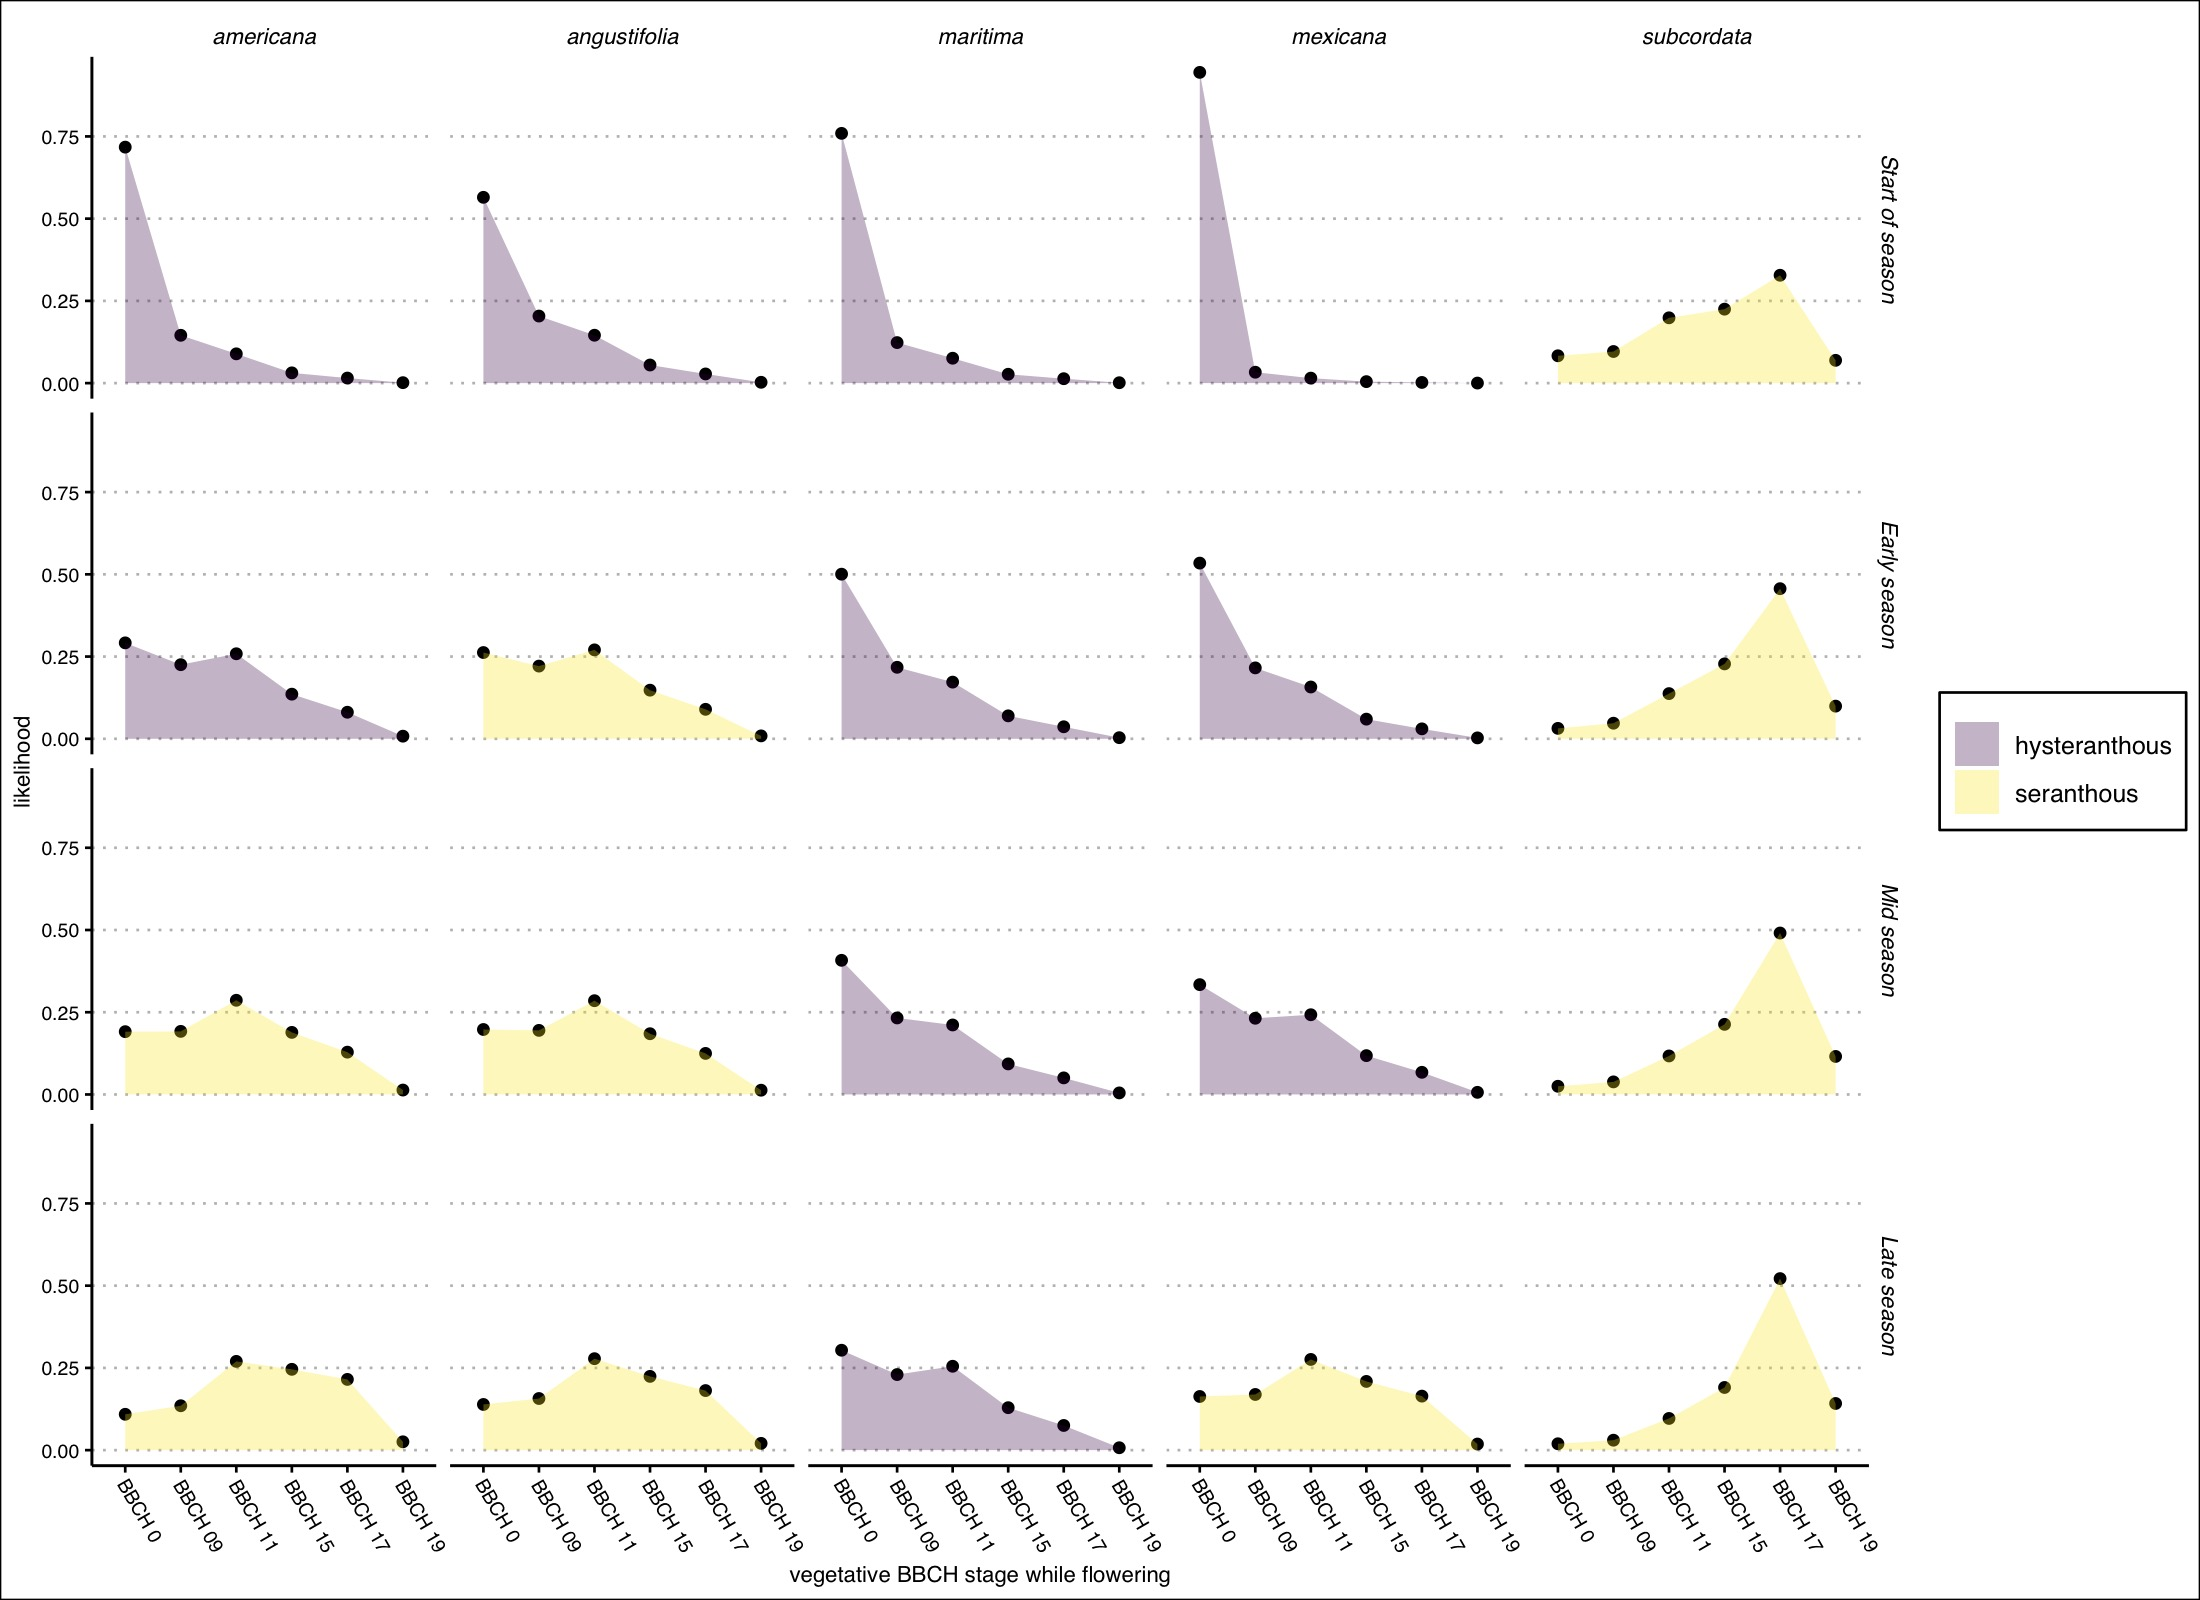
\includegraphics[width=\textwidth]{..//..//Plots/ord_quants_exmpsps.jpeg}
    \caption{Predicted likelihood that a species would be in flower during each vegetative BBCH phase for five example species in the American plums. Points are the mean likelihood and bar the 95\% uncertainty intervals. Species were classified as hysteranthous if greater than 50\% probability flowering occurred in BBCH 0 and BBCH 09 (colors) for each part of the flowering season.
  See Fig. \ref{fig:plums} for all species and alternative hysteranthy classification schemes. }
    \label{fig:ordinals}
\end{figure}




\begin{figure}[h!]
    \centering
 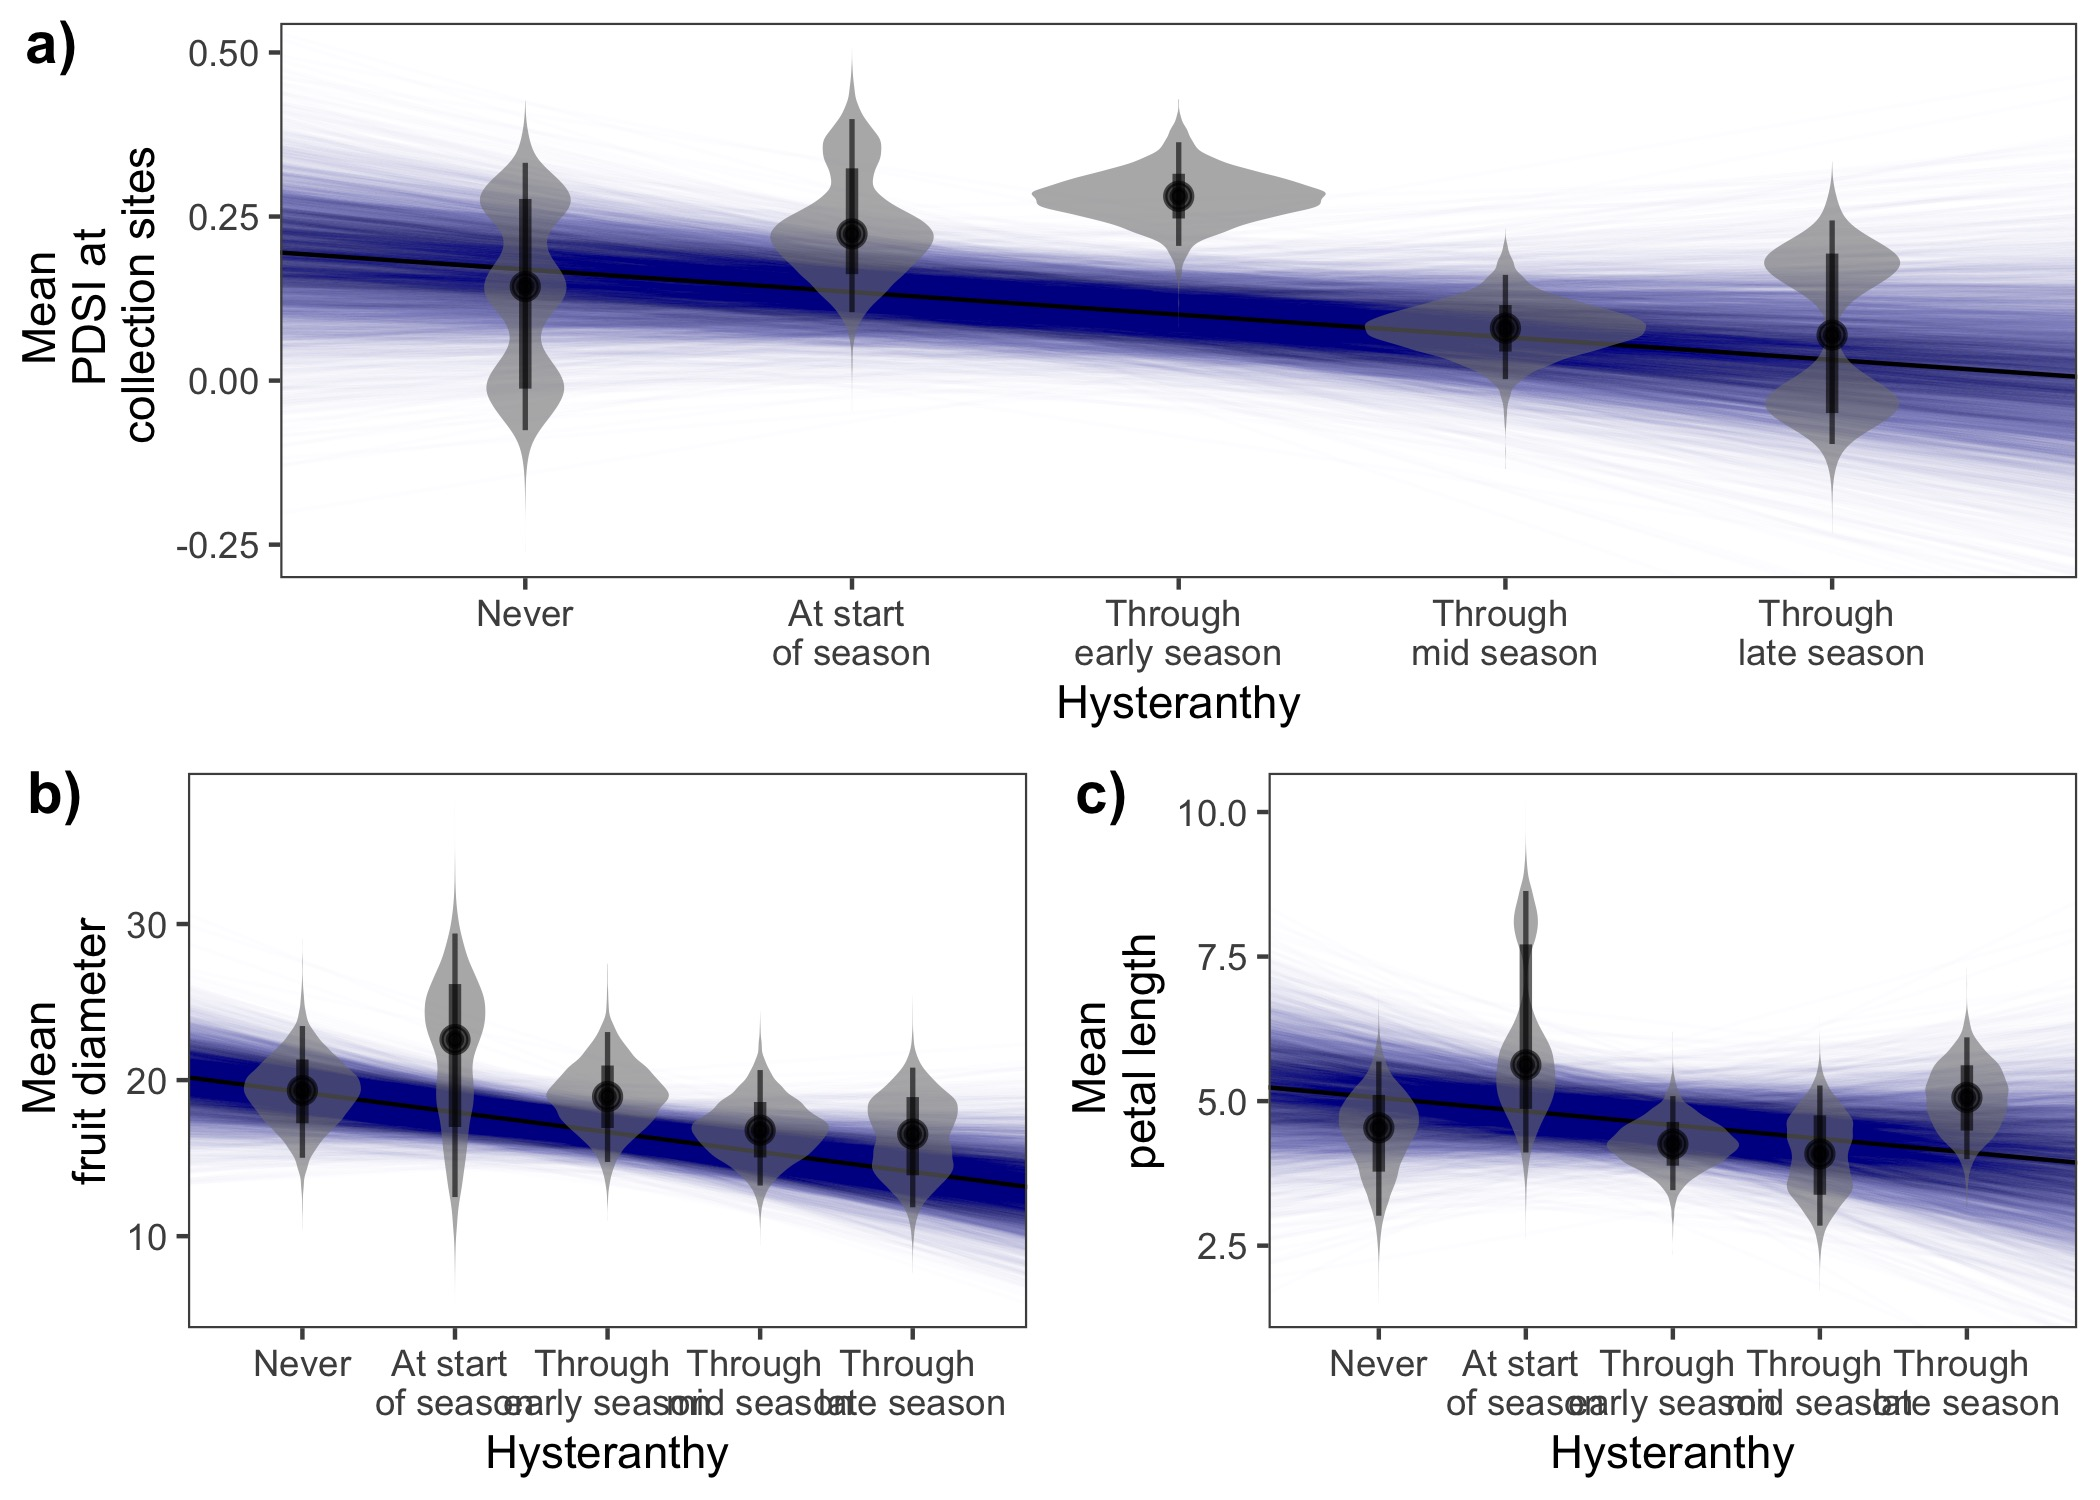
\includegraphics[width=\textwidth]{..//..//Plots/dataplots.jpeg}
    \caption{Relationships between the duration of hysteranthy across the flowering period and environmental and biological traits based on Bayesian phylogenetic mixed models. a) b) and c) dipict the relationships between the duration of hysteranthy and mean PDSI, fruit diameter, and petal length respectively. Solid lines indicate the mean posterior estimate and shaded areas X draws from the posterior distrubtion as a display of uncertainty. }
    \label{fig:prunes}
\end{figure}


\begin{figure}[h!]
    \centering
 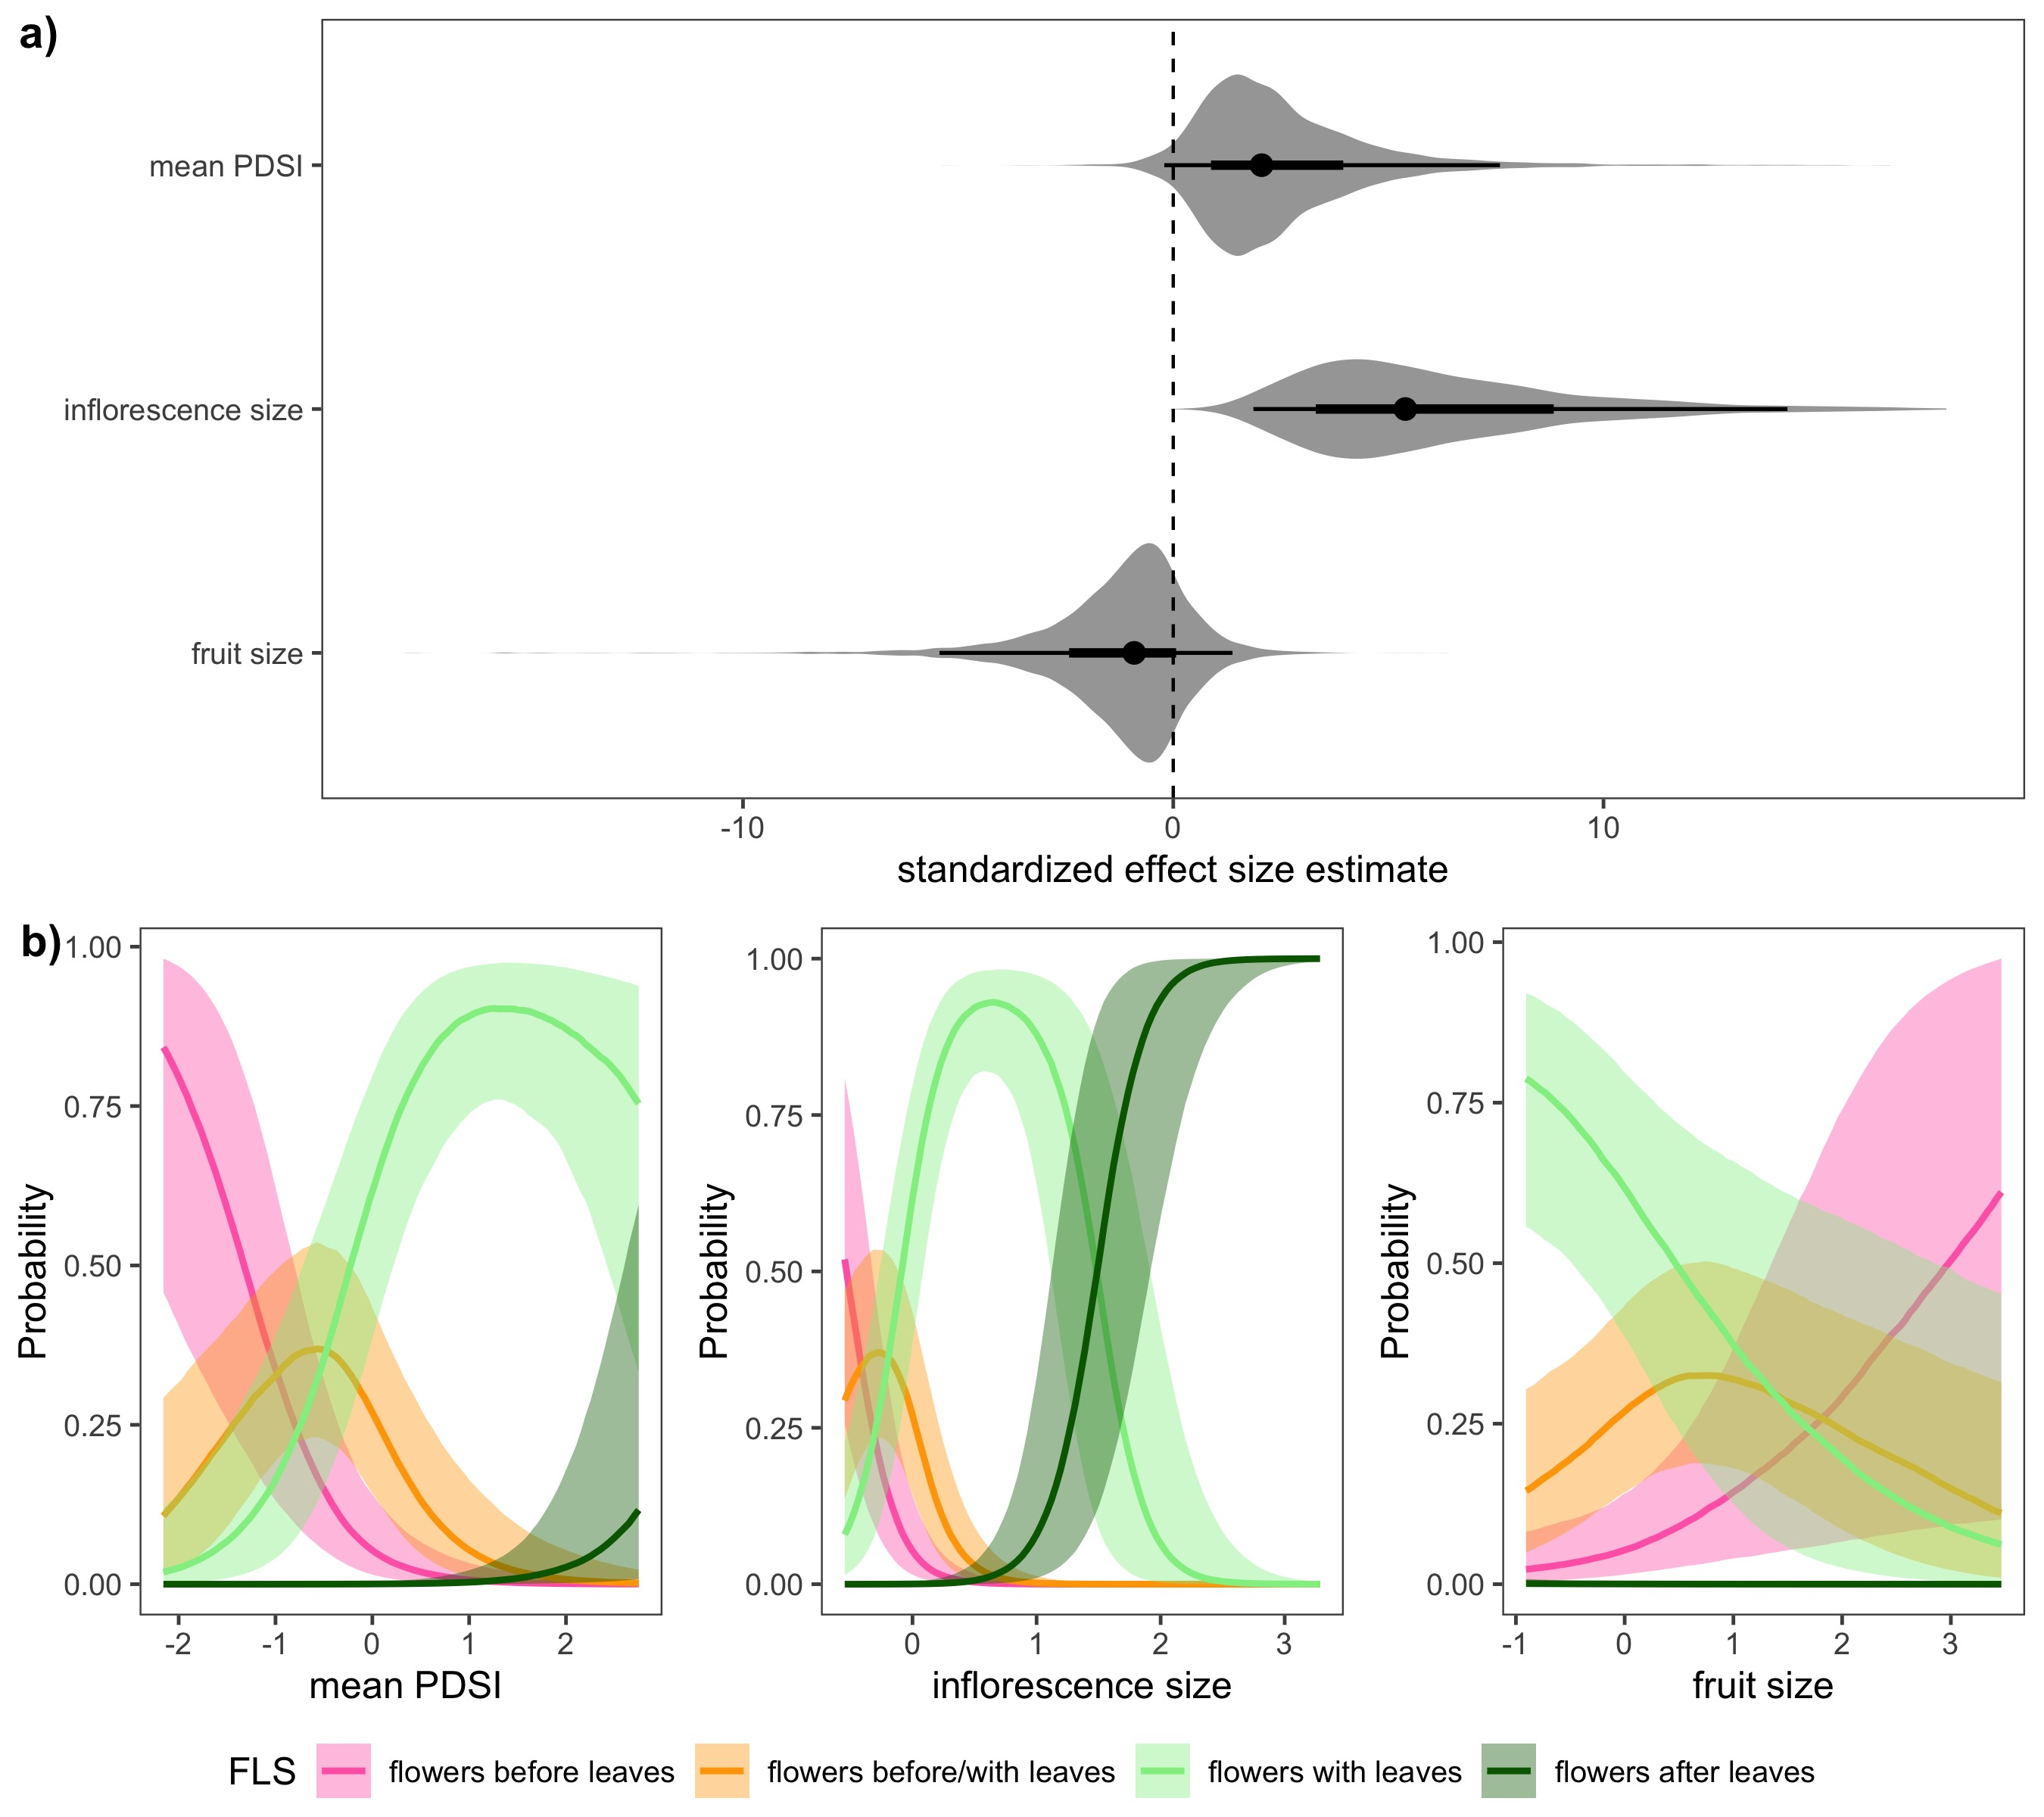
\includegraphics[width=\textwidth]{..//..//Plots/fullprunus_4manu.jpeg} %emwmar9 --mv fruit to supp?
    \caption{Relationships between the likelihood of of hysteranthy and environmental and biological traits in the genus Prunus based on Bayesian phylogenetic mixed models. Panel a) shows the estimated effect size of each predictor with negative values indicating an increased likelihood of hysteranthy. Points indicate the mean posterior estimate for each predictor, and thick and thin bars the 50\% and 97.5\% uncertaintly intervals respectively. We also show the full posterior distribution as an aditional meaure of uncertainty, Panel b), c) and d) show the marginal effect of mean PDSI, inflorescence size and fruit size respectively, on the likelihood that of each FLS category. Solid lines indicate the mean likelihood and shaded areas the 50\% uncertainty intervals.}
    \label{fig:genus}
\end{figure}


\end{document}
